\documentclass{beamer}
\mode<presentation>
\usepackage{amsmath,amssymb,mathtools}
\usepackage{textcomp}
\usepackage{gensymb}
\usepackage{adjustbox}
\usepackage{subcaption}
\usepackage{enumitem}
\usepackage{multicol}
\usepackage{listings}
\usepackage{url}
\usepackage{graphicx}
\def\UrlBreaks{\do/\do-}

\usetheme{Boadilla}
\usecolortheme{lily}
\setbeamertemplate{footline}{
\leavevmode
\hbox{
\begin{beamercolorbox}[wd=\paperwidth,ht=2ex,dp=1ex,right]{author in head/foot}
\insertframenumber{} / \inserttotalframenumber\hspace*{2ex}
\end{beamercolorbox}}
\vskip0pt
}
\setbeamertemplate{navigation symbols}{}

\lstset{
frame=single,
breaklines=true,
columns=fullflexible,
basicstyle=\ttfamily\tiny
}

\numberwithin{equation}{section}

\newcommand{\myvec}[1]{\ensuremath{\begin{pmatrix}#1\end{pmatrix}}}
\let\vec\mathbf

\title{Matgeo Presentation - Problem 2.5.2}
\author{Revanth Siva Kumar.D -- EE25BTECH11048}

\begin{document}

\begin{frame}
\titlepage
\end{frame}

\begin{frame}{Problem Statement}
Verify the type of triangle formed by the points:A(-4,0),B(4,0),C(0,3).
\end{frame}

\begin{frame}{Solution: Setup}
\begin{align*}
    \vec{A}=\myvec{-4\\0},\quad
\vec{B}=\myvec{4\\0},\quad
\vec{C}=\myvec{0\\3}
\end{align*}


Vectors:
\begin{align*}
    \vec{AB}=\vec{B}-\vec{A}=\myvec{8\\0},\quad
\vec{AC}=\vec{C}-\vec{A}=\myvec{4\\3},\quad
\vec{BC}=\vec{C}-\vec{B}=\myvec{-4\\3}
\end{align*}
\end{frame}

\begin{frame}{Solution: Right-Angle Check}
\textbf{Step 2: Check for Right-Angled triangle (perpendicular sides)}

Dot product should be 0.
\small
\begin{align}
\vec{B}-\vec{A} &= \myvec{8\\0}, &
\vec{C}-\vec{A} &= \myvec{4\\3}, &
(\vec{B}-\vec{A})^\top (\vec{C}-\vec{A}) = \myvec{8&0}\myvec{4\\3} = 32 \neq 0 \\
\vec{A}-\vec{B} &= \myvec{-8\\0}, &
\vec{C}-\vec{B} &= \myvec{-4\\3}, &
(\vec{A}-\vec{B})^\top (\vec{C}-\vec{B}) = \myvec{-8&0}\myvec{-4\\3} = 32 \neq 0 \\
\vec{A}-\vec{C} &= \myvec{-4\\-3}, &
\vec{B}-\vec{C} &= \myvec{4\\-3}, &
(\vec{A}-\vec{C})^\top (\vec{B}-\vec{C}) = \myvec{-4&-3}\myvec{4\\-3} = -7 \neq 0
\end{align}

Since no pair of sides is perpendicular, the triangle is not right-angled.
\end{frame}

\begin{frame}{Solution:Isosceles triangle check}
    \begin{align}
\text{Midpoint of } AB: \quad \vec{M} = \frac{\vec{A}+\vec{B}}{2} = \myvec{0\\0} \\
\vec{C}-\vec{M} = \myvec{0\\3}-\myvec{0\\0} = \myvec{0\\3} \\
\vec{B}-\vec{A} = \myvec{8\\0} \\
(\vec{B}-\vec{A})^\top (\vec{C}-\vec{M}) = \myvec{8&0}\myvec{0\\3} = 0
\end{align}


\begin{align*}
\text{Hence, } C \text{ lies on the perpendicular bisector of } AB.\\
AC = BC = 5 \implies \triangle ABC \text{ is isosceles.}
\end{align*}

\end{frame}

\begin{frame}{Conclusion}
Therefore, the triangle with vertices $(-4,0), (4,0), (0,3)$ is an \textbf{isosceles triangle} with $AC = BC = 5$.    
\end{frame}

\begin{frame}[fragile]{C Source Code: points.c}
\begin{lstlisting}[language=C]
#include <math.h>

// Compute dot product of 2D vectors
double dot_product(double *u, double *v) {
return u[0]*v[0] + u[1]*v[1];
}

// Compute squared norm of 2D vector
double norm_squared(double *u) {
return u[0]*u[0] + u[1]*u[1];
}
\end{lstlisting}
\end{frame}

\begin{frame}[fragile]{Python Script: call c.py}
\begin{lstlisting}[language=Python]
import ctypes
import numpy as np
import matplotlib.pyplot as plt

lib = ctypes.CDLL("./points.so")

lib.dot_product.argtypes = [ctypes.POINTER(ctypes.c_double),
ctypes.POINTER(ctypes.c_double)]
lib.dot_product.restype = ctypes.c_double

lib.norm_squared.argtypes = [ctypes.POINTER(ctypes.c_double)]
lib.norm_squared.restype = ctypes.c_double

A = np.array([-4.0, 0.0])
B = np.array([4.0, 0.0])
C = np.array([0.0, 3.0])

AB = B - A
AC = C - A
BC = C - B

dp1 = lib.dot_product(AB.ctypes.data_as(ctypes.POINTER(ctypes.c_double)),
AC.ctypes.data_as(ctypes.POINTER(ctypes.c_double)))
dp2 = lib.dot_product((-AB).ctypes.data_as(ctypes.POINTER(ctypes.c_double)),
BC.ctypes.data_as(ctypes.POINTER(ctypes.c_double)))
dp3 = lib.dot_product((-AC).ctypes.data_as(ctypes.POINTER(ctypes.c_double)),
(-BC).ctypes.data_as(ctypes.POINTER(ctypes.c_double)))
\end{lstlisting}
\end{frame}

\begin{frame}[fragile]{Python Script: call c.py}
\begin{lstlisting}[language=Python]
AB2 = lib.norm_squared(AB.ctypes.data_as(ctypes.POINTER(ctypes.c_double)))
AC2 = lib.norm_squared(AC.ctypes.data_as(ctypes.POINTER(ctypes.c_double)))
BC2 = lib.norm_squared(BC.ctypes.data_as(ctypes.POINTER(ctypes.c_double)))

print("Dot products:", dp1, dp2, dp3)
print("Squared lengths: AB^2 =", AB2, "AC^2 =", AC2, "BC^2 =", BC2)

plt.plot([A[0], B[0]], [A[1], B[1]], 'r-', label='AB')
plt.plot([A[0], C[0]], [A[1], C[1]], 'g-', label='AC')
plt.plot([B[0], C[0]], [B[1], C[1]], 'b-', label='BC')

plt.scatter([A[0], B[0], C[0]], [A[1], B[1], C[1]], color='black')
plt.text(A[0], A[1], 'A(-4,0)', ha='right', va='top')
plt.text(B[0], B[1], 'B(4,0)', ha='left', va='top')
plt.text(C[0], C[1], 'C(0,3)', ha='center', va='bottom')

plt.axis('equal')
plt.legend()
plt.grid(True)
plt.show()
\end{lstlisting}
\end{frame}

\begin{frame}[fragile]{Python Script: plot.py}
\begin{lstlisting}[language=Python]
import matplotlib.pyplot as plt
import numpy as np

A = np.array([-4, 0])
B = np.array([4, 0])
C = np.array([0, 3])

plt.plot([A[0], B[0]], [A[1], B[1]], 'r-', label='AB')
plt.plot([A[0], C[0]], [A[1], C[1]], 'g-', label='AC')
plt.plot([B[0], C[0]], [B[1], C[1]], 'b-', label='BC')

plt.scatter([A[0], B[0], C[0]], [A[1], B[1], C[1]], color='black')
plt.text(A[0], A[1], 'A(-4,0)', ha='right', va='top')
plt.text(B[0], B[1], 'B(4,0)', ha='left', va='top')
plt.text(C[0], C[1], 'C(0,3)', ha='center', va='bottom')

plt.axis('equal')
plt.legend()
plt.grid(True)
plt.show()
\end{lstlisting}
\end{frame}

\begin{frame}{Result Plot}
\begin{figure}[H]
\centering
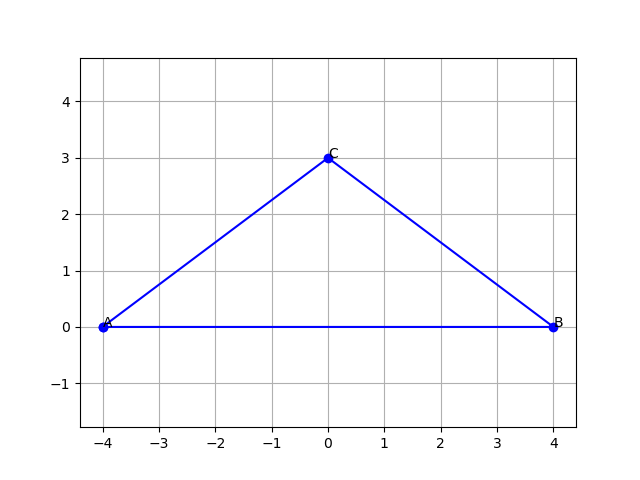
\includegraphics[width=0.7\columnwidth]{figs/Figure_1.png}
\caption*{Triangle $ABC$ plotted using shared output}
\end{figure}
\end{frame}
\begin{frame}{Result Plot}
\begin{figure}[H]
\centering
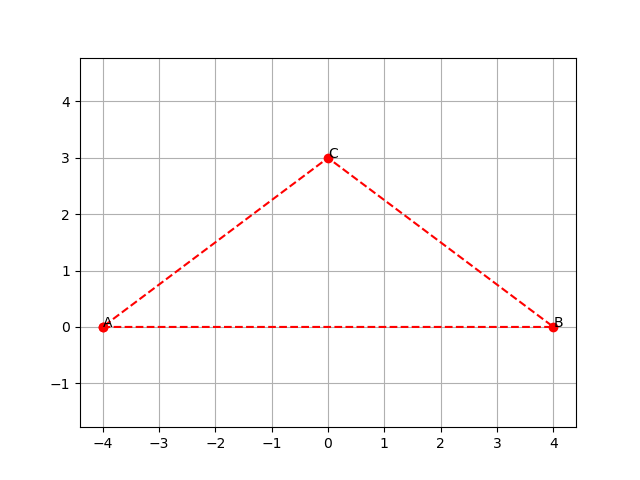
\includegraphics[width=0.7\columnwidth]{figs/Figure_2.png}
\caption*{Triangle $ABC$ plotted using direct python}
\end{figure}
\end{frame}
\end{document}
